\documentclass[extern,palatino]{cgBA}
\usepackage{setspace}
\usepackage{graphicx}
%\onehalfspacing
\doublespacing

\author{Martin Groppe und Malte Kremer}
\title{Entwicklung eines Augmented Reality-Rollenspiels für Android}
\zweitgutachter{...}
\externLogo{7.46cm}{logos/UniLogoNeu}
\externName{DIN: NewTechnologies}

\begin{document}

% Umschalten der Sprache (für englische Rubrikbezeichnungen etc.)
%\selectlanguage{english}


\maketitle

\newpage

\pagenumbering{roman}
\tableofcontents
\clearpage         % oder \cleardoublepage bei zweiseitigem Druck
% \listoffigures   % fuer ein eventuelles Abbildungsverzeichnis
% \clearpage
\pagenumbering{arabic}


\section{Abstract}

Das Mobile-Game Pokémon Go wurde in den ersten drei Monaten nach seiner dem Veröffentlichung 500 Millionen mal heruntergeladen, als Hybrid aus Rollen- und Augmented Reality-Spiel bleibt es aber eine Ausnahme. Außerdem hat es einige Schwächen.
\\Vor dem Hintergrund des großen Erfolges und der großen Begeisterung, die Pokémon Go ausgelöst hat, ist es Ziel dieser Arbeit, Pokémon Go und vergleichbare Produkte zu analysieren und gute Aspekte daraus aufzugreifen, um einen Prototypen für ein AR-Rollenspiel zu entwickeln. Dabei ist es unser Ziel, anders als Pokémon Go Spieltiefe und langfristigen Spaß stärker in den Vordergrund zu stellen.
Anschließend wird dieser von Testpersonen darauf geprüft, ob er Spaß macht und das Potenzial hätte, langfristig zu fesseln um allgemeine Erkenntisse über die Qualität des Prototypen zu gewinnen.
\section{Abstract (english)}
Pokémon Go was an enormous success, it was downloaded 500 million times in the first three months. Nevertheless it remains a rare case of a combination of Augmented reality and role-playing game features. It's also lacking in terms of actual depth and long time progression.
\\This thesis intends to develop a role-playing game on Android that uses Google Maps features for augmented reality purposes and is fun and engaging. Our goal is also to have more complexity in fights and to make continuous playing interesting. The implementation will then be tested and evaluated.
\newpage
\section{Motivation}
Spätestens seit dem massiven Erfolg von Pokémon Go sind Smartphones als Spieleplatform nicht mehr wegzudenken. Dennoch bleibt Pokémon Go eher eine Ausnahme insofern, als die AR-Möglichkeiten des Smartphones selten mit klassischen Spielkonzepten kombiniert wird. Dies ist vor dem Hintergrund überraschend, dass Pokémon Go gezeigt, dass es relativ einfach ist, Elemente der realen Welt in Rollenspiele zu integrieren. \\In der vorliegenden Arbeit haben wir es uns somit zum Ziel gesetzt zu erforschen, inwieweit es möglich ist, in einem relativ kurzen Zeitraum und mit geringem Budget einen Prototyp zu entwickeln, der AR-Elemente verwendet, kurzfristig Spaß macht und das Potenzial hat langfristig zu fesseln.
\newpage
\section{Grundlagen}
Da das Spiel auf dem Betriebssystem Android laufen soll, wurde die Entscheidung gefällt, Interface und Basis-Programm in java zu programmieren. Als Entwicklungsumgebung für den java-Code wird Google's hauseigenes Android Studio verwendet, da es gut dokumentiert und weit verbreitet ist.
\\Die Kämpfe hingegen werden mit der Unity-game-engine erstellt, sodass für die Erstellung der Grafik nur ein Bildbearbeitungsprogramm benötigt wird. Dazu wird Adobe Photoshop verwendet.
\subsection{Android}
\subsubsection{AR-Funktionen von Android}
\newpage
\subsection{Unity}
Unity, eine von Unity Technologies entwickelte Game engine ist seit ihrer Veröffentlichung 2005 zunehmend erfolgreich. %laut wikipedia nutzen 47% der Spiele auf mobilen Geräten unity.
Sie wird von Indie-Entwicklern wie William Chyr Studios ebenso wie von Publisher-abhängigen Entwicklungsstudios wie z.B. Square Enix Montreal benutzt. Unity ermöglicht einfache Entwicklung für die Smartphone-Betriebssysteme iOS, Android, Windows Phone, aber auch für Computer-Betriebssysteme und für Konsolen wie die Playstation 4 oder den 3DS.
\\Insgesamt sind mit Unity über 238.000 Spiele\footnote{[Quelle: unity analytics]} für den mobilen Markt %(Quelle: unity analytics) 
und etwa 34\% der Top 1.000 mobilen Spiele entwickelt worden, es ist die meistbenutzte nicht-inhouse-Engine. Allein im dritten Quartal 2016 hatte Unity über fünf Milliarden downloads. Außerdem ist es benutzerfreundlich und gut dokumentiert. Darüber hinaus vereinfacht die große Verbreitung den Einstieg zusätzlich.
\\Unity bietet die Möglichkeit in 2D sowie in 3D zu programmieren und bietet übersichtliche objektorientierte Verknüpfungen von Scripts und Game-Objekten. Unitys Script Compiler arbeitet mit C\# oder JavaScript. Darüber hinaus hat es Automatismen für die Erstellung von Animationen aus Basis-Data wie 3D-Modellen oder Spritesheets. 
\newpage 
\subsection{Photoshop}
Das Bildbearbeitungsprogramm Photoshop wurde 1988 von Adobe entwickelt. Seitdem wurden mehrfach neue Versionen entwickelt. Mit Photoshop werden Bilder auf Pixel-basis bearbeitet. Dies ermöglicht relativ einfache Erstellung von sogenannten Sprites, also Bildern die als Basis für 2D-Figuren dienen.
\\
Photoshop ist in unter Game-Artists weit verbreitet und wird für die Erstellung von Storyboards, Sketches und Sprites benutzt. Animation Career Review listet es als die essenziellste Software für Künstler und Designer, Developer hat es in ihrer nicht-sortierten 'Top acht'-Liste, bloopanimation empfiehlt es ebenfalls für 2d-Animation und bezeichnet es als "großartige Wahl ("great choice"). 2005 lag Photoshops' Marktanteil zwischen 60\% und 70\% im Bereich Bildbearbeitungssoftware für Rastergrafik (Bundeskartellamt, %http://www.bundeskartellamt.de/SharedDocs/Entscheidung/DE/Entscheidungen/Fusionskontrolle/2005/B7-162-05.pdf?\_\_blob=publicationFile\\&v=3
), 2010 hatte Photoshop über 10 Millionen Nutzer weltweit.
\\
Außerdem ist das Programm gut dokumentiert und leicht zu lernen (eine Google-Suche nach Photoshop Tutorial lieferte rund 14.500.000 Ergebnisse). All diese Faktoren machten es zu einer guten Wahl für die Erstellung der Grafik.
\newpage

\section{Recherche von Rollenspiel und AR-Hybriden auf Android}
\subsection{Pokémon Go}
Pokémon Go ist ein freemium/free-to-play Smartphone-Spiel für iOS und Android. Es wurde von Niantic im Juli 2016 veröffentlicht und benutzt Google Maps sowie situational das Gyroskop und die Kamera für AR-Funtionen. 
\\Pokémon Go ist bis heute das erfolgreichste Spiel, das für Smartphones erschienen ist, mit über 650 Millionen Downloads (Stand 27.02.2017) und über 500 Millionen Downloads in den ersten zwei  Monaten.%http://archive.is/XCgwL
2016 haben gleichzeitig an einem Tag 23 Millionen Nutzer gespielt.
\\
Im Folgenden wird grob die Funktionsweise von Pokémon Go erklärt. Pokémon Go benutzt GPS, um die Position der Spieler zu erfassen und auf einer Google Maps-ähnlichen Karte anzuzeigen. Niantics' Server erzeugt Pokémon (Monster, die man fangen, trainieren und zum kämpfen benutzen kann) an mehr oder weniger zufälligen realen GPS-Positionen. Dabei berücksichtigt der Server eine Reihe von Faktoren. Pokémon vom Typ 'Wasser' werden z.B. eher in der Nähe von Flüssen, Seen und Brunnen erschaffen, während Pokémon vom Typ 'Geist' eine erhöhte Chance haben, bei Nacht aufzutauchen. Wenn der Spieler nah genug an ein Pokémon heran kommt, kann er das Pokémon sehen und auf es tippen, um einen Bildschirm aufzurufen, in dem er versuchen kann, es mit einem Pokéball zu fangen. Sollte es dem Spieler nicht gelingen, dass Pokémon innerhalb einer bestimmten Zeit zu fangen, entkommt es.
\\Außerdem gibt es an festgelegten Orten sogenannte Poké-Stops, an denen Spieler Items wie die bereits erwähnten Pokébälle bekommen können. Zusätzlich gibt es Arenen, an denen Spieler gegen die Pokémon von anderen Spielern kämpfen können um Items zu bekommen. Dies führt dazu, dass Spieler häufig in der realen Welt bestimmte Routen ablaufen und sich an festgelegten Orten immer wieder begegnen, was mehr oder weniger automatisch zu neuen Kontakten und Freundschaften führt. Neben den realen Kontakten, mit denen man das Spiel spielen kann, und den Orten, die man besucht, sorgt auch die Kamera-Anzeige, in der Pokémon vor einem realen Hintergrund angezeigt werden und die Anpassung von Pokémon in Gebieten für eine Verknüpfung von realer und virtueller Welt. 
\\Das Spiel ist kostenlos herunterladbar, im Shop kann man z.B. Pokébälle oder Inventar-Erweiterungen für eine Ingame-Währung kaufen, die man auch mit realem Geld kaufen kann. Nutzer die reales Geld ausgeben, haben dementsprechend Vorteile, die einen schnelleren Fortschritt ermöglichen. Laut Schätzungen hat Pokémon Go 2016 etwa 950 Millionen US-Dollar Einnahmen erzeugt.%https://venturebeat.com/2017/01/17/pokemon-go-generated-revenues-of-950-million-in-2016/
\\Auch wenn Pokémon Go alle Smartphone-Spiel-Rekorde gebrochen hat, gibt es doch einige Kritik. Die Interaktionsmöglichkeiten mit anderen Spielern hielten sich stark in Grenzen, das Monetisierungs-Modell war recht unterentwickelt und es gab kein wirklich forderndes Element. Arena-Kämpfe erwiesen sich als recht repetetiv und anspruchslos und echtes Player versus Player-Gameplay, bei dem beide Seiten aktiv Einfluss auf das Kampfgeschehen nehmen können, gibt es nicht. Es gibt auch keinen anderen fordernden Endgame-Inhalt, sodass viele Spieler Pokémon erst trainierten, schließlich aber feststellen mussten, dass sie nicht viel mit den trainierten Pokémon machen konnten. %http://archive.is/bFBtX
\newpage
\subsection{Parallel Kingdom}
Das von PerBlue 2008 auf den Markt gebrachte Parallel Kingdom war ein Smartphone-Spiel, das Elemente aus MMORPG-, Geocache-Spielen und von Real-time browser-based MMOs wie OGame beinhaltete. Es lief server-basiert und wurde im November 2016 abgeschaltet. 
\\Das Spiel beinhaltete verschiedene MMO-Elemente, OGame-Features und Geo-Features. So konnte man z.B. Ressourcen und Items sammeln und tauschen, Dungeons erforschen und Monster bekämpfen. Das Spiel spielte  auf einer realen Weltkarte, auf der man sich (im Gegensatz zu Pokémon Go und unserem Spiel) auch virtuell fortbewegen konnte und Territorium beanspruchen konnte. OGame Features wie Gebäuden, die stetigen Ertrag bringen und PvP-Kriege um Gebiete boten zusätzliche Langzeitmotivation.
\\Das Spiel war mit über 1.000.000 Spielern recht erfolgreich, wurde mehrfach für Awards nominiert und hatte mit acht Jahren eine für ein Android Spiel sehr lange Lebensdauer.  %https://www.nowgamer.com/parallel-kingdom-interview-when-mmo-meets-gps/
Die Abschaltung war laut Entwickler hauptsächlich wegen der veralteten Technik notwendig. %http://www.parallelkingdom.com/community/update-hut.aspx#302
Die lange Zeit, über die das Spiel lief, zeigt, dass die Konzepte gut ineinander griffen und es genug Inhalte gab, um Spieler auf lange Sicht zu fesseln. PerBlue machte mehrere große Updates, die zusätzliche Features und Gebiete brachten. Leider waren viele Bereiche im Kern recht simpel, Kämpfe bestanden häufig daraus, dass Spieler nebeneinander liefen und anschließend Schläge tauschten. Am Ende wurden sie oft durch Items und Level entschieden und nicht von den Entscheidungen der Spieler. Als wir anfingen, das Spiel zu testen, war es bereits wenige Monate vor der Abschaltung und Fortschritt war in dem Spiel recht langsam, sodass wir nicht dazu kamen, die großen PvP-Funktionen zu testen, da die Nutzerzahl schon stark geschrumpft war.
\subsection{Motion Tennis Cast}
In dem 2007 veröffentlichten Motion Tennis Cast spielt man Tennis mit seinem Smartphone. Das Spielkonzept ist ähnlich wie der Tennis-Teil von Wii Fit, das Smartphone dient als Controller und wird mit einem Fernseher oder Computer verbunden, der dann als Bildschirm dient. Dabei benutzt das Spiel die Bewegungssensoren des Smartphones für Motion Capturing und der Spieler simuliert mit seinem Smartphone Schläge mit einem Tennisschläger. Leider benötigt das Spiel zusätzliche Software und laut User-Reviews ist das Game instabil und ungenau.
\newpage

\section{Recherche von Rollenspielen auf dem PC und auf Konsolen}
\subsection{klassische Rollenspiele}
Klassische Rollenspiele wie die Final Fantasy-Serie aus Japan, die Witcher-Serie oder Bioware-Spiele wie Knights of the Old Republic oder Baldur's Gate legen meistens einen großen Fokus auf eine gute Geschichte und ein lebendiges virtuelles Umfeld. Zusätzlich stehen häufig Erkundung und gelegentlich kleinere Rätsel im Vordergrund, während Kämpfe und Items eher im Hintergrund stehen. 
\\Das Genre nähert sich wieder zunehmend den Open-World-Titeln an, Spielen ihren Spielern durch große virtuelle Gebiete ohne Ladezeiten das Gefühl von Freiheit geben. So besaßen sowohl der dritte Teil der Witcher-Reihe The Witcher 3: Wild Hunt (2015) als auch der dritte Teil von Bioware's Dragon Age Serie Dragon Age: Inquisition (2014) eine frei begehbare Welt und das Open-World-Spiel The Elder Scrolls 5: Skyrim (2011) hatte ausgereiftere Levelmechaniken, eine bessere Präsentation seiner Geschichte und mehr Dialog-Sprecher (83) als seine Vorgänger. %http://www.imdb.com/title/tt3763912/fullcredits?ref_=tt_cl_sm#cast %http://www.statisticbrain.com/skyrim-the-elder-scrolls-v-statistics/
%https://en.wikipedia.org/wiki/Horizon_Zero_Dawn#Development
\subsection{Open-World Titel und MMORPGs}
Open-World-Spiele setzen den Spieler in eine riesige, frei erkundbare Welt. Dabei ist zu unterscheiden zwischen Einzelspieler-Spielen wie der Elder Scrolls Serie (zuletzt The Elder Scrolls 5: Skyrim (2011)) und sogennanten MMORPGs wie World of Warcraft (2004, letzte Erweiterung 2016), Spielen in denen oft hunderte Spieler auf dem gleichen Server in der gleichen Instanz der Welt spielen. Da unser Spiel allerdings ein AR-Spiel sein sollte, war die Kreirung einer großen virtuellen Welt für uns eher uninteressant, außerdem ziehen MMORPGs oft ihren Reiz aus der Interaktion mehrerer Spieler miteinander, was eine gute abschließende Auswertung erschweren würde.
\subsection{Action-Rollenspiele}
Action-RPGs wie die Diablo-Serie von Blizzard, Titan Quest, die Sacred-Reihe oder das Freemium-Spiel Path of Exile konzentrieren sich eher auf schnelles Gameplay mit viel Action. Der Held erlebt in der Regel eine eher oberflächliche Geschichte und besiegt hunderte Feinde in effektgeladenen Kämpfen. Dabei sorgt ein stetiger Strom an Gegnern für einen guten Spielfluss. Langzeit-Motivation wird häufig durch zufällig generierte Items, Klassen mit unterschiedlichen Fähigkeiten und Mehrspieler-Inhalte erzeugt.
\subsection{Taktik-Rollenspiele}
Taktik-Rollenspiele sind Rollenspiele, in denen man ein eher strategisches Gameplay hat. In Spielen wie der Disgaea-Serie, der Final Fantasy Tactics-Reihe oder der Fire Emblem-Serie spielt man rundenbasiert größere Gruppen auf Schachbrett-artigen Feldern. Dabei hat jede Figur Items und ein eigenes Level und gehört häufig einer Klasse an, die eigene Stärken und Schwächen mit sich bringt. So können Magier in der Regel über größere Distanzen viel Schaden anrichten, sind aber eher sehr gefährdet wenn Gegner an sie herankommen. Der 2014 erschienene Indie-Titel The Banner Saga fällt ebenfalls in diese Kategorie.
\subsubsection{Final Fantasy Tactics}
Das 1997 veröffentlichte Playstation-Spiel Final Fantasy tactics und sein 2003 erschienener Nachfolger für den Gameboy Advance sind Klassiker unter den Taktik-Rollenspielen. Ausgereifte und komplexe Level- und Klassensysteme sorgen für viele Möglichkeiten bei der Charakter-Entwicklung und für Langzeitmotivation und die Kämpfe sind immer ein bisschen anders. Stil und Grafik sind bei beiden Titeln gut, aber während Final Fantasy Tactics eine ausgereifte und komplexe Geschichte hat, steht diese bei Final Fantasy Tactics Advance eher im Hintergrund.
\subsubsection{The Banner Saga}
The Banner Saga ist ein von Stoic entwickeltes Taktik-Rollenspiel. Es wurde von drei ehemaligen BioWare-Mitarbeitern produziert, die über Crowdfunding Geld gesammelt haben, um ihr Projekt zu finanzieren. Banner Saga wurde über Steam und GOG.com (Good old Games) vertrieben und wurde alleine in Steam über 600.000 mal verkauft.
\\In Banner Saga spielt man zwei Gruppen, die versuchen in einem apokalyptischen Szenario zu überleben. Banner Saga orientiert sich in Stil und Handlung stark an der nordischen Mythologie im allgemeinen und an Ragnarök, dem Weltuntergang. Eine Gruppe besteht hauptsächlich aus sogenannten Varls, gehörnte Riesen, die versuchen zu ihrer Hauptstadt zu kommen, während die andere Gruppe aus hauptsächlich aus menschlichen Flüchtlingen besteht und nach Süd-Westen zieht, um der Invasion der sogenannten Dredge aus dem Norden zu entkommen.
Banner Saga erzählt eine tragische Handlung, die vom Spieler beeinflusst werden kann. Kämpfe werden auf einem Schachbrett ausgetragen und Figuren besitzen Spezialfähigkeiten, die im Laufe des Spiels stärker werden. 
\subsection{Strategie-Rollenspiel-Hybriden} Spiele wie die Heroes of Might and Magic- oder die Disciples Serie sind eher im Strategie-Bereich als im Rollenspiel-Sektor anzusiedeln, haben aber starke Rollenspiel-Komponenten. So haben diese Spiele, anders als die vorher erwähnten Taktik-Rollenspiele Basen, in denen man Truppen baut und eine Weltkarte, über die man frei zieht, allerdings wird der Anführer der Armee im Laufe des Spieles ebenfalls stärker und kann Items finden und in Disciples bekommt auch die Armee Erfahrung.

\newpage
\section {Konzeption}
\subsection{Frühe Konzeption}
Unsere ersten Konzepte legten, ähnlich wie Pokémon Go, einen stärkeren Fokus auf Augmented Reality. Ursprünglich sollte der Spieler eine einzelne Figur steuern und z.B. mithilfe von Motion-Capturing mit Gesten in der Realität Fähigkeiten innerhalb eines Rollenspiels ausführen. So wollten wir uns im Kampfsystem stärker an Action-Rollenspielen orientieren, was auch Mehrspieler-Modi ermöglicht hätte.
\\Unsere Recherche hat allerdings ergeben, dass bisher existierende Beispiele für Motion Capturing mit dem Smartphone durch Ungenauigkeiten Probleme verursachen und das Projekt wahrscheinlich viel Feinabstimmung bräuchte, sodass es fragwürdig war, ob innerhalb von sechs Monaten ein vorzeigbares Ergebnis zu schaffen ist. Außerdem brauchten wir einen zweiten portablen Bildschirm, andernfalls müsste der Spieler zwischen seinen Bewegungen und dem Blick auf das Smartphone abwechseln, was allerdings den Spielfluss zu stark belasten würde. Das einzige Motion-Capturing Android Spiel, dass das Smartphone wie eine Wiimote (Wii-Controller) benutzte, erforderte für diesen Zweck einen Fernseher oder einen Laptop. Diese Lösung erlaubt jedoch kaum Mobilität.
\\Vorstellbar wäre ein solches Konzept, wenn die Smartphone-VR-Technologie und die Smart-Watch weiter entwickelt wären, aber selbst dann wäre es schwer bis unmöglich, innerhalb von sechs Monaten einen gut funktionierenden Prototyp zu kreiren, solange Motion-Capturing nicht von einem anderen Programm übernommen wird.
\\Daher fokussierten wir uns eher auf anspruchsvolles Gameplay und funktionierende Rollenspiel-Systeme als eine stärkere AR-Anbindung. Dazu war es sinnvoll, sich Rollenspiele auf anderen Plattformen stärker anzusehen und zu überlegen, welche Ideen wir übernehmen und erweitern können.
\newpage
\subsection{Zweite Konzept-Phase}
Klassische Rollenspiele haben in der Regel mehrere Storywriter und Sprecher, was im Rahmen einer Bachelor-Arbeit mit zwei Personen nicht produzierbar ist. Außerdem fehlt uns Erfahrung im Schreiben größerer Geschichte mit vielen Charakteren. Daher entschieden wir uns, einen Hybriden aus den Stärken anderer Subgenres zu erzeugen, der in absehbarer Zeit produzierbar ist und gleichzeitig Spaß macht. 
\\Unsere Kämpfe orientieren sich an denen von Taktik-Rollenspielen, da einer der großen Kritikpunkte an Pokémon Go die mangelnde Spieltiefe war und Kämpfe in Taktik-Rollenspiele durch ihr Schachbrett oft Tiefe erzeugen, ohne so hektisch wie die von Action-Rollenspielen zu sein. \\Tests zeigten, dass Kämpfe in Taktik-Rollenspielen zwar durchaus lange dauern konnten, diese in den Taktik-Rollenspielen sehr ähnlichen Rollenspiel-Strategiespiel-Hybriden wie die Heroes of Might and Magic-Serien aber unter einer Minute liegen konnten, also immernoch unterwegs gut spielbar wären. Die längere Dauer in Spielen wie Fire Emblem oder Disgaea liegt häufig an der Spielfeldgröße und der größeren Menge an Kampfteilnehmern (in der Fire Emblem Serie können durchaus 40 Charaktere an einer Schlacht teilnehmen). Da wir aber schnelle Kämpfe benötigen, damit Spieler nicht nur auf der Stelle stehen und kämpfen,  sondern auch immer wieder weitergehen, entschieden wir uns für mehrere Optimierungen. So wird die Anzahl an Kampfteilnehmer sowie das Schlachtfeld klein zu halten und Schaden ist im Verhältnis zu Lebenspunkten relativ hoch, sodass Kämpfe nach ungefähr drei Runden vorbei sind. Um den Strategiefaktor nicht zu vernachlässigen und das Spiel komplex zu halten, entschieden wir uns für mehrere Klassen mit verschiedenen Stärken und Schwächen.
\\Level- und Itemsysteme werden dagegen stärker an Action-Rollenspielen und MMORPGs angelehnt. Items sollen eine Motivationsquelle für Spieler sein und für ein zusätzliches Belohnungsgefühl und für ein Gefühl des stärker werdens sorgen. Aufgrund des zeitlichen Rahmens ist es uns jedoch nicht möglich, zahlreiche Unikate zu erschaffen. Daher werden unsere Items automatisch generiert, kommen aber in verschiedenen Seltenheitsstufen und Leveln. Unser Ziel war es, dass seltene Items große Vorteile bringen, damit Spieler sich freuen, wenn sie sie bekommen.
\\Zusätzlich sieht unser Konzept ein Questsystem vor, welches Spieler Belohnungen gibt und sie dazu motivieren soll, sich ihre Kämpfe genauer auszusuchen. Dabei unterteilen wir in eine kleine und eine große Quest, während die kleine Quest in der Regel innerhalb einer Stunde erledigbar sein soll, wird die große Quest dazu gedacht sein, Spieler über einen längeren Zeitraum zu beschäftigen. Dadurch wird für eine gewisse Langzeit-Motivation gesorgt.
\\Die Optik soll sich dabei an Taktik-Rollenspielen und Strategie-Rollenspiel-Hybriden orientieren, wobei versucht wird, anders als Pokémon stärker erwachsenes und westliches Publikum zu erreichen, da unser Spiel stärker auch Langzeit-Spieler ansprechen soll. Gleichzeitig soll das Spiel aber weiterhin für junges Publikum spielbar bleiben.  \\In Tests sorgten 3D-Modelle insbesondere bei Animationen häufig für Ecken an Stellen die eigentlich rund sein sollten, sodass jedes Keyframe einer Animation erneut nachbearbeitet werden musste. Daher wurde sich für 2D-Sprites und gegen 3D-Modelle entschieden, da diese in relativ kurzer Zeit bessere Ergebnisse lieferten.
\newpage
\section{Implementierung}
Die Implementierung umfasste mehrere verschiedene Teilaspekte und Sprachen, sowie das Erstellen von Grafik und Menüs, wobei Martin sich hauptsächlich auf die Android Seite und das eigentliche Kampfmodul konzentrierte und Malte auf die Grafik, Design-Entscheidungen und die Erstellung des Siegesbildschirms in Unity.
\\Die App wurde nach und nach modular erzeugt. So wurde am Anfang der Fokus auf den Unity-Teil gelegt, in dem unser Kampf abläuft. Dabei übernahm Martin die Programmierung des Schachbrettes, der Figuren, der Wegfindung und der künstlichen Intelligenz, während Malte sich auf Stil und Grafik konzentrierte. Beide waren an allen Kernentscheidungen beteiligt.
\subsection{Erstellung des Kampfes in Unity}
In Unity werden Gameobjects als Basiseinheit für die Erstellung von Spielen verwendet. Gameobjects sind Behälter denen man verschiedene Komponenten wie Sprites und Skripte hinzufügen kann. Für die Steuerung unseres rundenbasierten Kampfes generieren wir in Unity ein Gitter aus Quadraten die sich anklicken lassen und ihre Position im Gitter kennen. Damit der Kampf sich nicht immer gleich anfühlt erzeugen wir zufällig auf unseren Quadraten Steine als Hindernisse. Unsere Spielfiguren werden dann abhängig davon welche am Kampf beteiligt sind aus sogenannten Prefabs, Schablonen aus denen man ein Gameobject instanziieren kann, erzeugt und auf die Seiten des Spielfeldes gesetzt. Figuren sind nun reihum am Zug. Wenn eine Figur die dem Spieler gehört an der Reihe ist markieren wir alle Felder zu denen sie sich bewegen kann auf unserem Feld. Wird eines dieser Felder angeklickt generieren wir wie in \ref{Pfadfindung} beschrieben einen Pfad den unsere Figur dann abläuft. In unseren Prefabs sind die zugehörigen Animationen für die verschiedenen Befehle vorgemerkt. Wenn der Benutzer auf eine gegnerische Figur in Reichweite der aktiven klickt wird diese angegriffen und der Zug beendet. Alternativ kann man die aktive Figur anklicken um den Zug ohne Angriff zu beenden. Wenn die aktive Figur dem Gegner gehört übernimmt eine simple Ai die Entscheidungen die sonst der Spieler trifft. Die Ai überprüft ob eine feindliche Figur in Reichweite ist und greift diese an fals möglich. Wenn nicht bewegt sie sich auf die nächste feindliche Figur auf dem Feld zu. Falls sie nun in Reichweite ist greift sie die Figur an andernfalls beendet sie ihren Zug.
\subsection{A* Pfadfindung}\label{Pfadfindung}
Um Figuren auf unserem Spielfeld zu bewegen benötigen wir einen Suchalgorithmus um einen Pfad zu finden. Wir haben dazu den A* Algorithmus implementiert. Im Gegensatz zu uninformierten Suchalgorithmen wie Dijkstra wird in A* eine Heuristik benutzt um Zielgerichtet zu suchen. Alle Felder werden in 3 Gruppen unterteilt. Die erste Gruppe sind die noch nicht gefundenen Felder. Am Anfang sind dies alle außer dem Startfeld. Die 2. Gruppe sind die Felder zu denen mindestens ein Weg bekannt ist. Diese werden zusammen mit einem Wert f(x) in einer Liste gespeichert. Der Wert von f(x) ergibt sich aus der Summe der Kosten um den Knoten zu erreichen g(x) und den geschätzten Kosten um von dort zum Ziel zu kommen. Im Falle von unserem Spiel kostet es einen Punkt um sich orthogonal zu bewegen und 2 diagonal. Die Schätzfunktion nimmt einfach die Summe der Abstände in x und y Koordinate zwischen einem Feld und dem Zielfeld. Zusätzlich wird für jedes Feld in dieser sogenannten Open List gemerkt von welchem Feld ausgehend der momentane Weg dort ankommt. Die 3. Gruppe besteht aus den Feldern zu denen bereits ein optimaler Weg gefunden wurde. Diese Felder werden in der sogenannten Closed List ebenfalls mit dem Feld von dem der kürzeste Weg zu ihm ausgeht gespeichert.
Zu Beginn befindet sich nur das Startfeld in der Open List und die Closed List ist leer. Nun wird in jedem Schritt das Feld x mit dem geringsten f-Wert aus der Open List in die Closed List aufgenommen. Für jedes Nachbarfeld y wird nun g(y) berechnet aus g(x)+1, falls es ein orthogonaler Nachbar, und g(x)+2 , falls es ein diagonaler Nachbar ist. Zusammen mit der oben beschriebenen Heuristik wird nun f(y) = g(y)+h(y) berechnet und y wird in die Open List mit x als Vorgänger aufgenommen, falls es dort nicht schon mit einem gleichgroßen oder kleineren f-Wert vorhanden ist. Der Algorithmus endet sobald das Zielfeld in der Open List aufgenommen wird. Der Weg ergibt sich nun indem man über die gemerkten Vorgänger die Felder bis zum Start zurückverfolgt.
\subsection{Karte und Menüs auf Android}
Unser Android Code besteht aus 4 Activities. Eine Activity in Android ist eine Oberfläche in der beschrieben wird was momentan angezeigt wird und wie mit Benutzereingaben umzugehen ist. Um zwischen den Activities zu kommunizieren werden sogenannte Intents verwendet. Unsere Hauptactivity auf der der Benutzer startet besteht aus 3 Fragmenten zwischen denen man mit swipen hin und her tauschen kann. In der Mitte befindet sich unsere Karte. Auf unserer Karte wird die Position des Spielers, die über Gps abgerufen wird, und die Position von Gegnergruppen gegen die man kämpfen kann angezeigt. Wird eine Gegnergruppe angeklickt wird ein Infofenster mit näheren Informationen zu den Gegnern angezeigt über das wenn man nah genug dran ist den Kampf starten kann. Die notwendigen Daten für den Kampf werden als Json Strings serialisiert und der Unity-Player-Activity über den Intent mitgeteilt.
\begin{figure}[htb] 
	\centering
	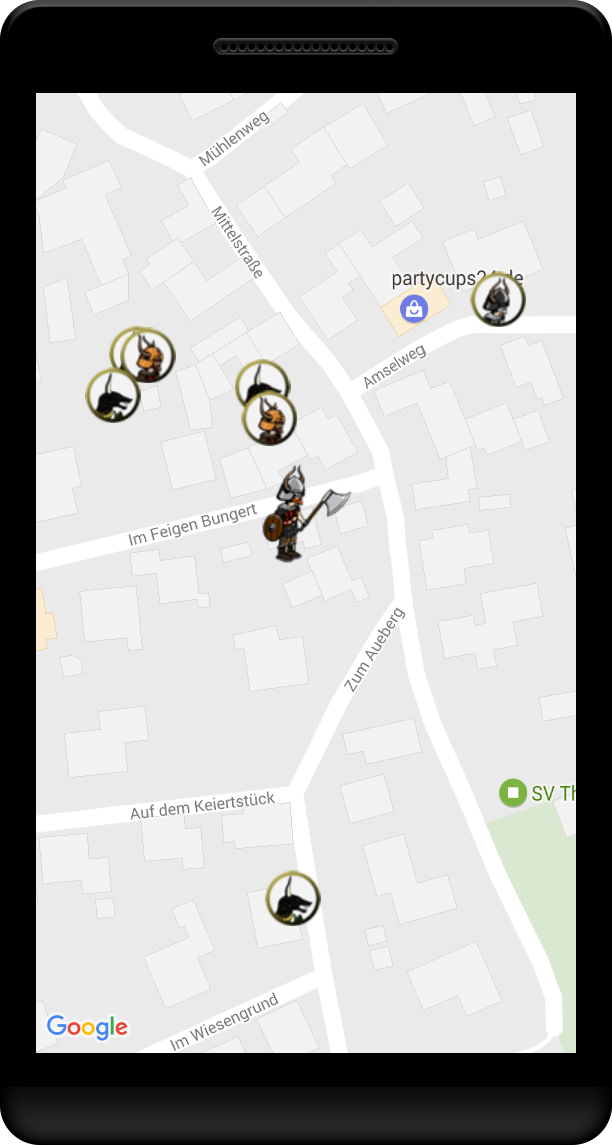
\includegraphics[width=0.4\textwidth]{map.png}
	\caption{Karte mit Spielfigur in der Mitte. Die Portraits representieren Gegnergruppen}
	\label{fig:Bild1}
\end{figure}
Im linken Fragment befindet sich unser Gruppen-Bildschirm. Auf ihm wird dem Spieler die eigene Gruppe angezeigt und er kann auswählen welche Charaktere am Kampf teilnehmen sollen. Die Charaktere in der oberen Leiste sind momentan aktiv und man kann sie indem man sie anklickt gegen einen beliebigen inaktiven Charakter austauschen.\begin{figure}[htb] 
	\centering
	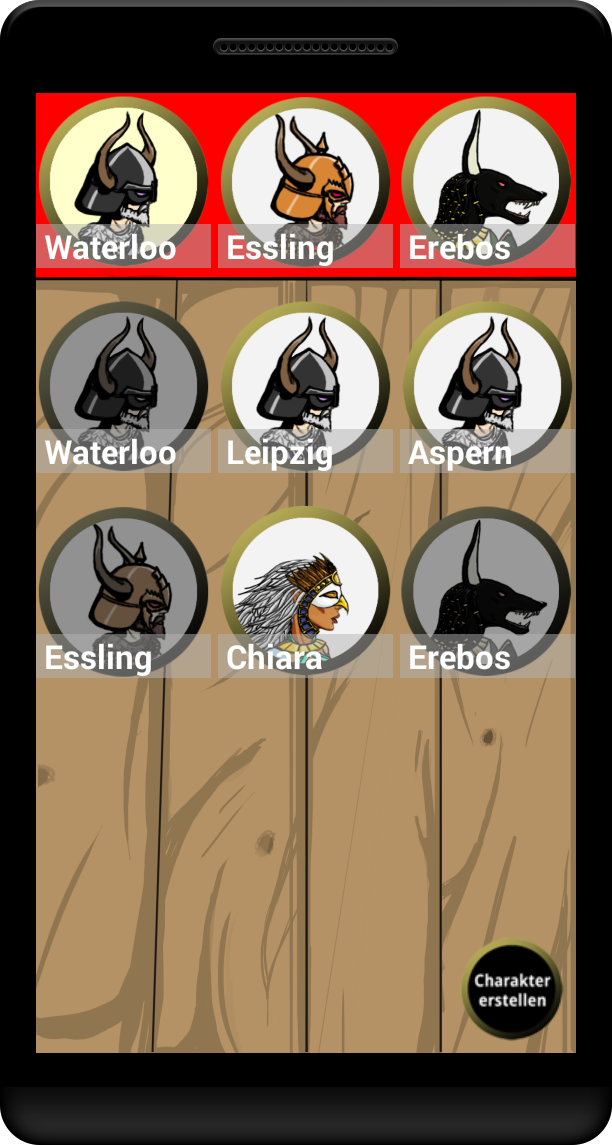
\includegraphics[width=0.4\textwidth]{charfragment.png}
	\caption{Charakter Fragment. Die aktive Party ist in der roten Leiste. Waterloo wurde angeklickt um ihn auszutauschen. Die möglichen Ziele für den Tausch sind Leipzig und Aspern}
	\label{fig:Bild2}
\end{figure} 
Wenn man auf einen Charakter im unteren Teil klickt werden die Daten des Characters in einen Intent gepackt und die StatusActivity (wir müssen unsere Bildschirme im Text besser benennen ersetze durch was du willst) wird gestartet. Über den Button unten rechts gelangt man zur Charaktererstellungs-Activity.
\newpage
Im rechten Fragment befindet sich eine Anzeige für momentane Aufgaben die der Spieler erfüllen kann um zusätzliche Belohnungen zu erhalten. Wenn der Spieler die Aufgabe erfüllt hat kann er diese über den Button abgeben und er bekommt einen zufälligen Gegenstand auf dem Level seiner Gruppe als Belohnung.
\newpage
\begin{figure}[htb] 
	\centering
	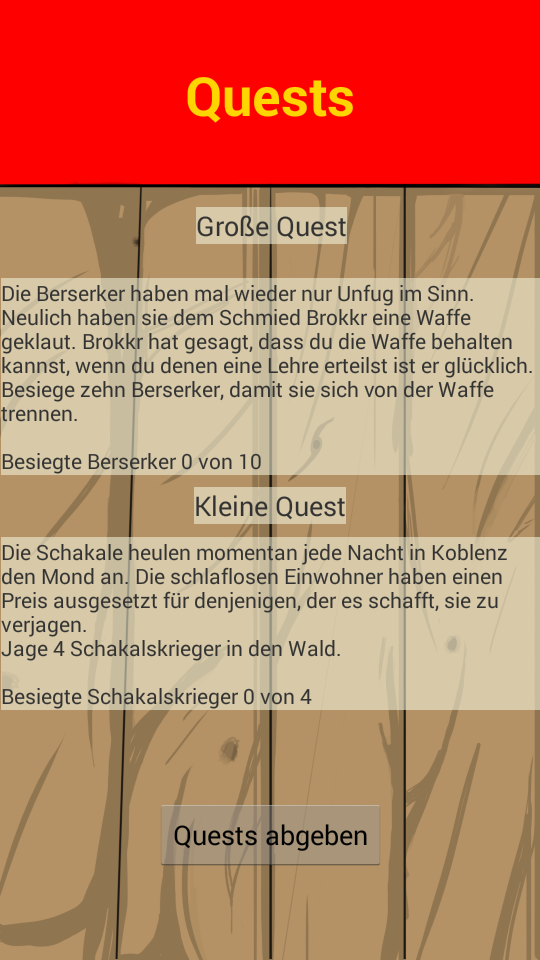
\includegraphics[width=0.4\textwidth]{questfragment.png}
	\caption{Questfragment mit momentan aktiven Aufgaben}
	\label{fig:Bild3}
\end{figure} 
Die zweite Activity ist die Unity-Player-Activity. In ihr kann der von Unity kompilierte Code abgespielt werden. Um zwischen Java und Unity-Code zu kommunizieren verwenden wir Java Native Interface, kurz JNI. JNI ist eine Programmierschnitstelle die es uns erlaubt von Unity aus Java Funktionen aufzurufen, die sich in unserer Unity-PLayer-Activity befinden. Wir benutzen JNI um die Kampfinformationen, die der Activity mitgeteilt werden, im Unity-Code abzurufen und um nachdem der Kampf fertig ist zurück zur MainActivity zu kommen.

Die dritte Activity ist die Statscreen-Activity. Hier werden die Statuswerte der Figur, die sie aufgerufen hat, angezeigt. Außerdem kann man hier der Figur gefundene Gegenstände anziehen um ihre Statuswerte zu verbessern.
\newpage
\begin{figure}[htb] 
	\centering
	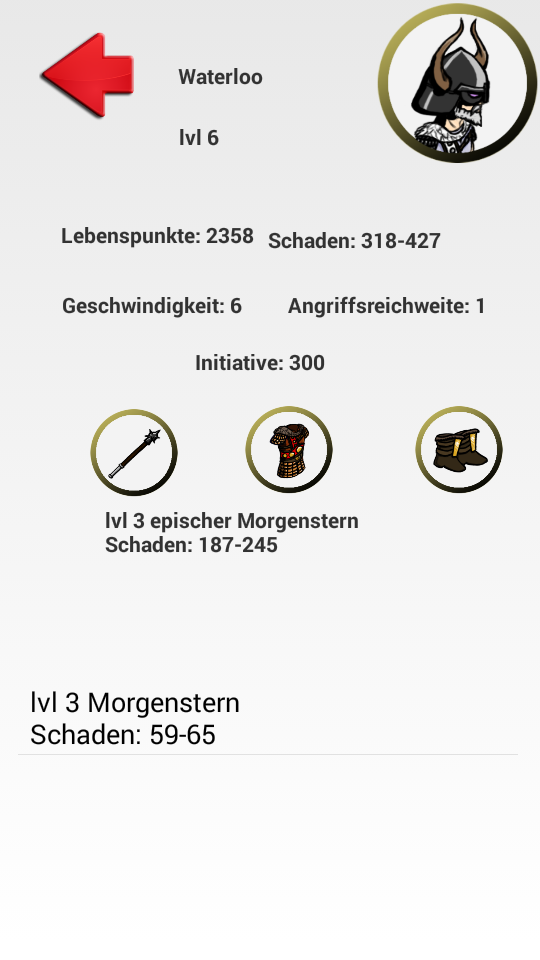
\includegraphics[width=0.4\textwidth]{statscreen.png}
	\caption{Statusbildschirm von Waterloo. Unten kann man die momentan ausgerüstete Waffe austauschen. Über die drei Symbole kann man zwischen Waffen, Rüstungen und Schuhen wechseln.}
	\label{fig:Bild4}
\end{figure} 

In der vierten Activity kann man sich eigene Charaktere erstellen. Über die vier Bilder kann man die Klasse des Charakters aussuchen und über das Textfeld einen Namen eingeben.
\newpage
\begin{figure}[htb] 
	\centering
	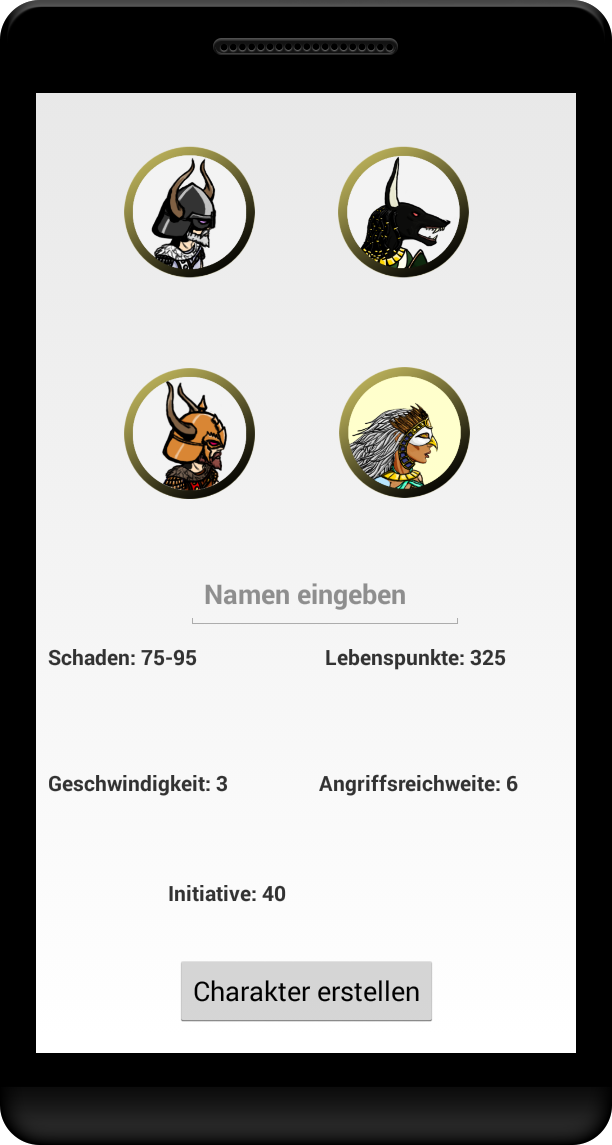
\includegraphics[width=0.4\textwidth]{createcharscreen.png}
	\caption{Hier kann man einen neuen Charakter erstellen.}
	\label{fig:Bild5}
\end{figure} 
\subsection{Grafik und Stil}
Der Stil sollte sowohl auf Smartphones als auch auf Tablets gut aussehen, ein breites Publikum ansprechen und sich vom normalen etwas abheben. Das hieß, dass es mehrere Probleme zu lösen gab:
\\1. Die größten Tablet-Bildschirme wie die vom Google Pixel C können über 25cm Bildschirmdiagonale haben, während unser Test-Smartphone z.B. gerade mal 11cm hat. Unser Spiel sollte also auf 13cm hohen Bildschirmen erkennbar sein, auf 30cm breiten Bildschirmen aber immer noch gut aussehen. Realistischere Darstellungen (Abb.1) waren auf dem Test-Smartphone  nicht gut erkennbar (Abb.2), sodass sich für einen Comic-Look mit unrealistischen Proportionen entschieden wurde. Dabei galt die Balance zu halten zwischen zu stark unterschiedlichen Proportionen, was insbesondere ältere Spieler häufig abschreckt, und Erkennbarkeit.
\begin{figure}
%	\raggedleft
	\centering
	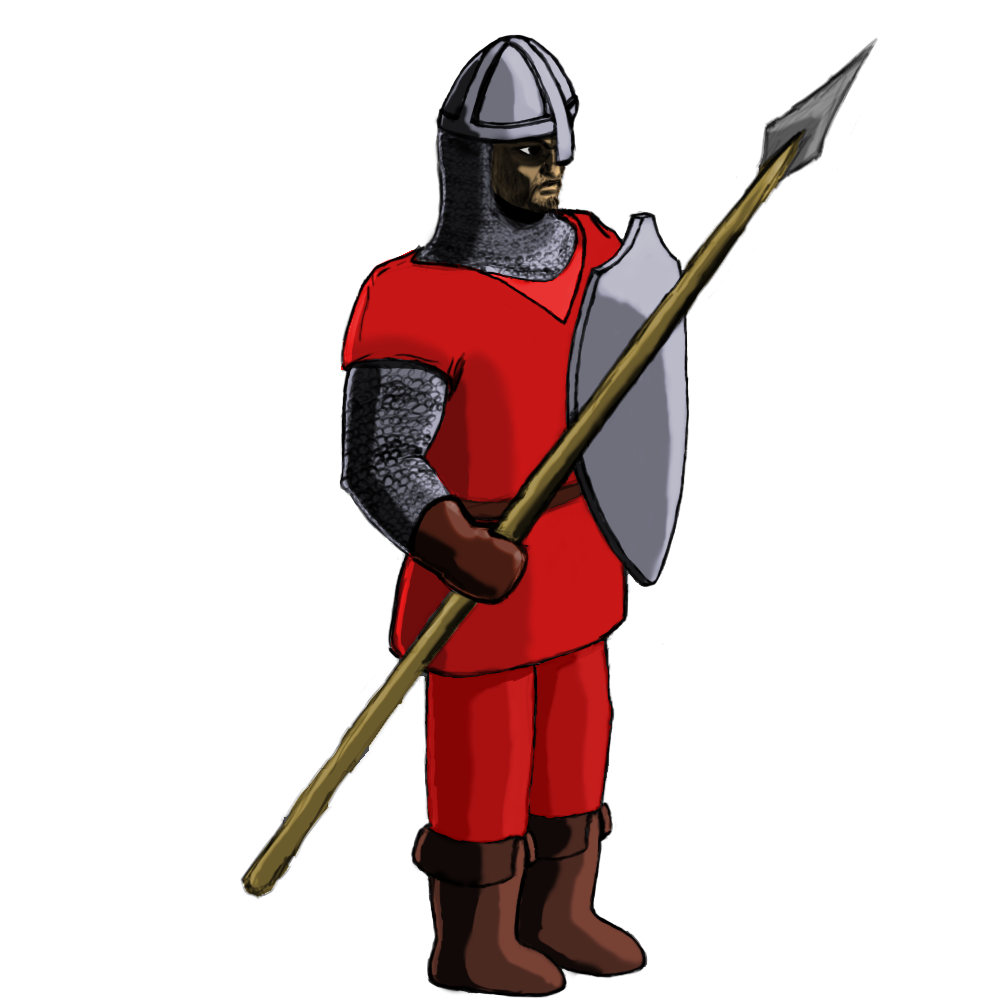
\includegraphics[height=5cm]{soldier.png}
	\caption{früher Entwurf eines Speerträgers}
\end{figure}
\begin{figure}
	\centering
	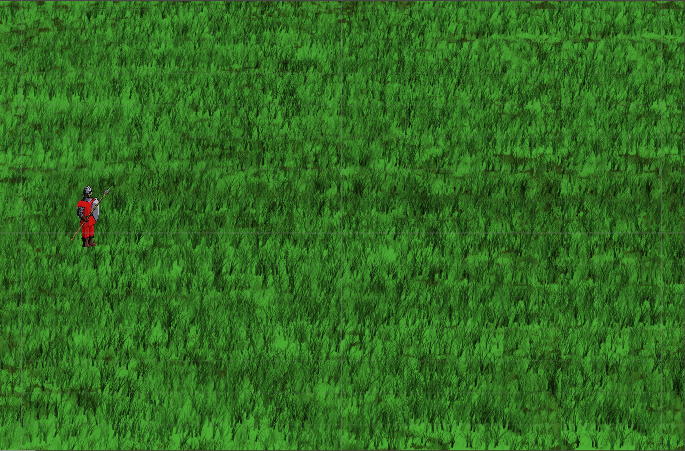
\includegraphics[width=13cm]{soldierbackground.png}
	\caption{Speerträger auf unserem Schlachtfeld}
\end{figure}
\\2. Das Spiel sollte Erwachsene und Jugendliche anziehen, aber immernoch bedenkenlos von Kindern spielbar sein. Das hieß, dass der Grafikstil nicht zu düster sein durfte, aber auch nicht zu kindisch, ohne generisch zu wirken.
\\3. Die hohe Detaildichte, welche bei die Entwicklung für Tablets erforderlich ist, erfordert einen hohen Zeitaufwand. Folglich mussten Animationen vom Grundmodell aus einfach zu erzeugen sein und eine Ansicht gewählt werden, in der das nicht stark auffällt.
\\Die meisten Taktik-Rollenspiele haben sehr abwechslungsreiche und häufig eher zufällige Karten und teils zufällige Startpositionen mit verschiedenen Terrain-Höhen. Da allerdings unser Fokus stärker auf strategischen als zufälligen Kämpfen lag, entschieden wir uns bei dem Aufbau des Schlachtfeldes für ein flaches Feld mit Gegnern auf der einen und Spielern auf der anderen Seite, wie es in Strategie-Spielen wie Schach oder der Heroes-Serie zum Einsatz kommt. Dies erleichterte auch das Grafikdesign, da Figuren sich hauptsächlich auf der horizontalen Achse bewegen, sodass eine 3/4-Ansicht mit situationaler Spiegelung für fast alle möglichen Lauf-Richtungen gut aussieht. Zusätzlich wurde sich entschieden, das Feld breiter als hoch zu machen, was auf das Gameplay positive Auswirkungen hatte, aber auch bedeutete, dass zum einen das Schlachtfeld besser der 16:9-Auflösung der meisten Smartphones entspricht, zum anderen die optisch schlechter aussehenden Bewegungen nach gerade oben oder gerade unten seltener sind.
\\Danach wurden mehrere Skizzen erstellt, um eine geeignete Balance zwischen realistisch und übertrieben/Comic-Look zu finden. Erste Versuche (s. Abb.3) waren stärker überzeichnet und an den sogenannte Chibi-Zeichenstil angelehnt, da ein vergrößerter Kopf leicht auszumachen ist und eine gute Differenzierung verschiedener Figuren ermöglichte. Es gab allerdings Bedenken, dass dies Hardcore-Spieler abschrecken könnte, die wir ansprechen wollten. Daher wurde der Kopf etwas weniger überzeichnet, der restliche Körper etwas normaler proportioniert und zusätzlich die Bewaffnung etwas vergrößert. Da geplant war, einige Figuren umzufärben, einige Details abzuändern und diese dann als neues Modell zu benutzten, erlaubte eine größere Waffe eine gute Erkennbarkeit von Elementen, die für Statuswerte wichtig sein sollten. So sollte es für den Spieler intuitiv verständlich sein, dass die Figur mit dem Schild mehr Schaden aushält und die Figur mit den zwei Äxten mehr Schaden macht, was bei purem Umfärben häufig ein Problem darstellt.
\begin{figure}
	%	\raggedleft
	\raggedleft
	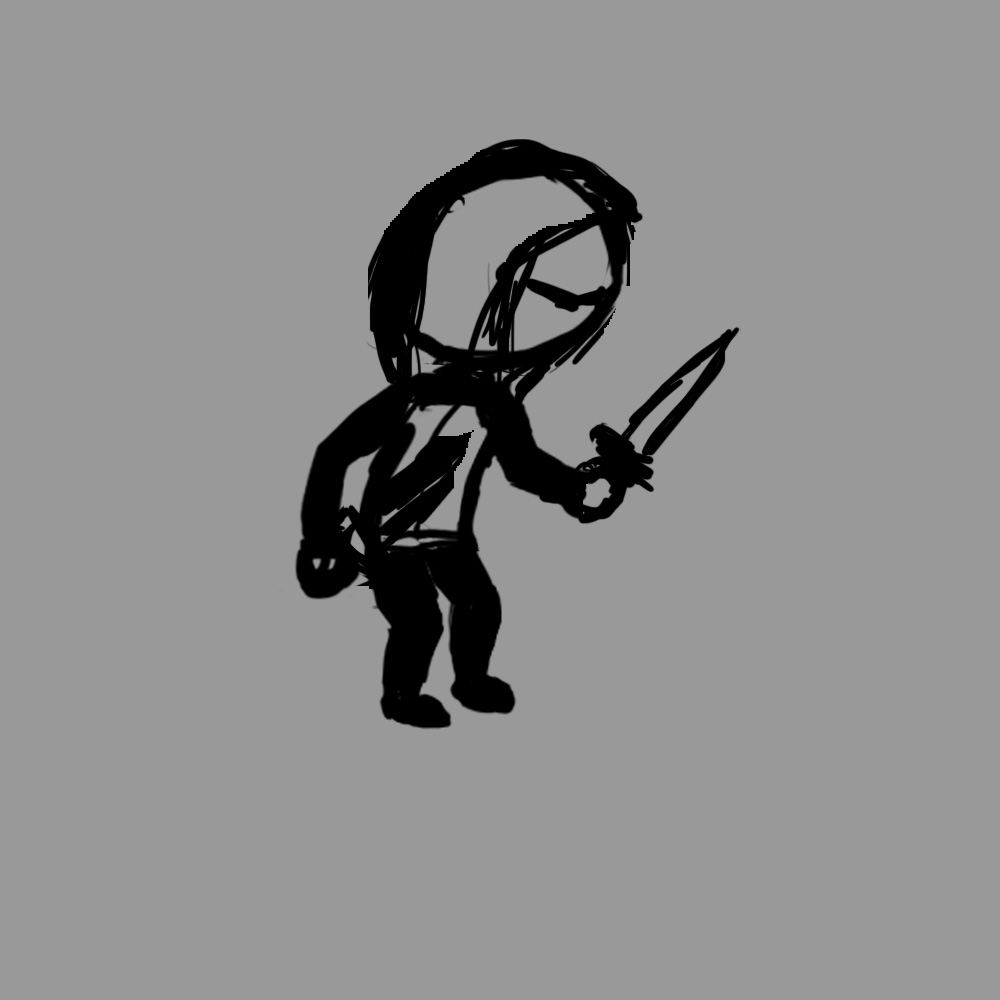
\includegraphics[width=5cm]{assachibi.jpg}
	\raggedright
	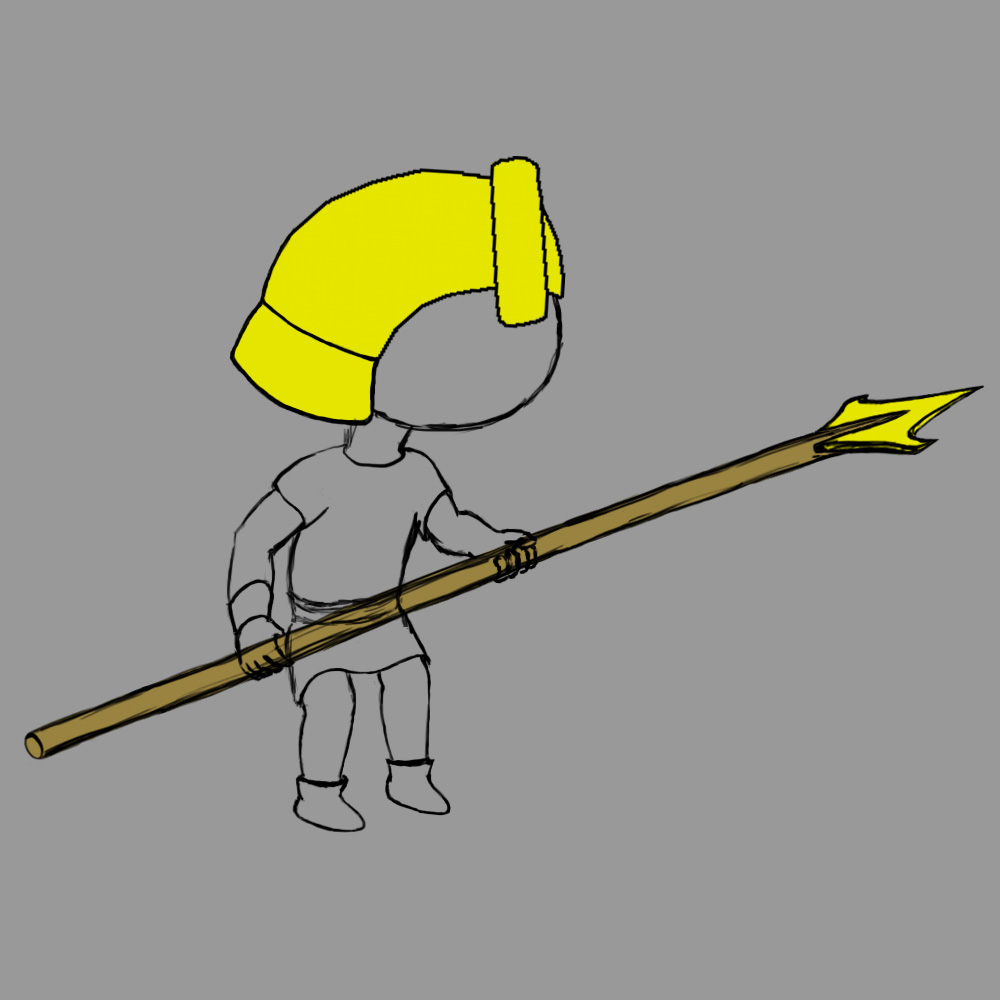
\includegraphics[width=5cm]{egychibi.jpg}
	\caption{frühe Entwürfe}
\end{figure}
\subsection{Die Figuren}
\begin{figure}
	\centering
	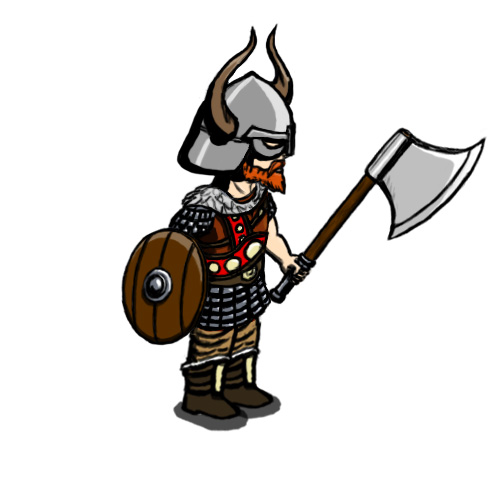
\includegraphics[height=8cm]{viking.jpg}
	\caption{der finale Wikinger}
\end{figure}
\subsubsection{Der erste Wikinger}
Da die klassischen Fantasy-Skizzen zu kindlich oder zu generisch gerieten, wurde bei den Motiven zunehmend weniger Mainstream-Motive verwandt. So wurde sich für ein Wikinger-Motiv entschieden, was es erlaubte, eine Figur düster und trotzdem niedlich aussehen zu lassen. Außerdem sind die gehörnten Helme in Medien ikonisch (wenn auch historisch falsch), sodass Spieler auch auf sehr kleinen Bildschirmen erkennen sollten, dass es sich um einen Wikinger handelt.
\begin{figure}
	\raggedleft
	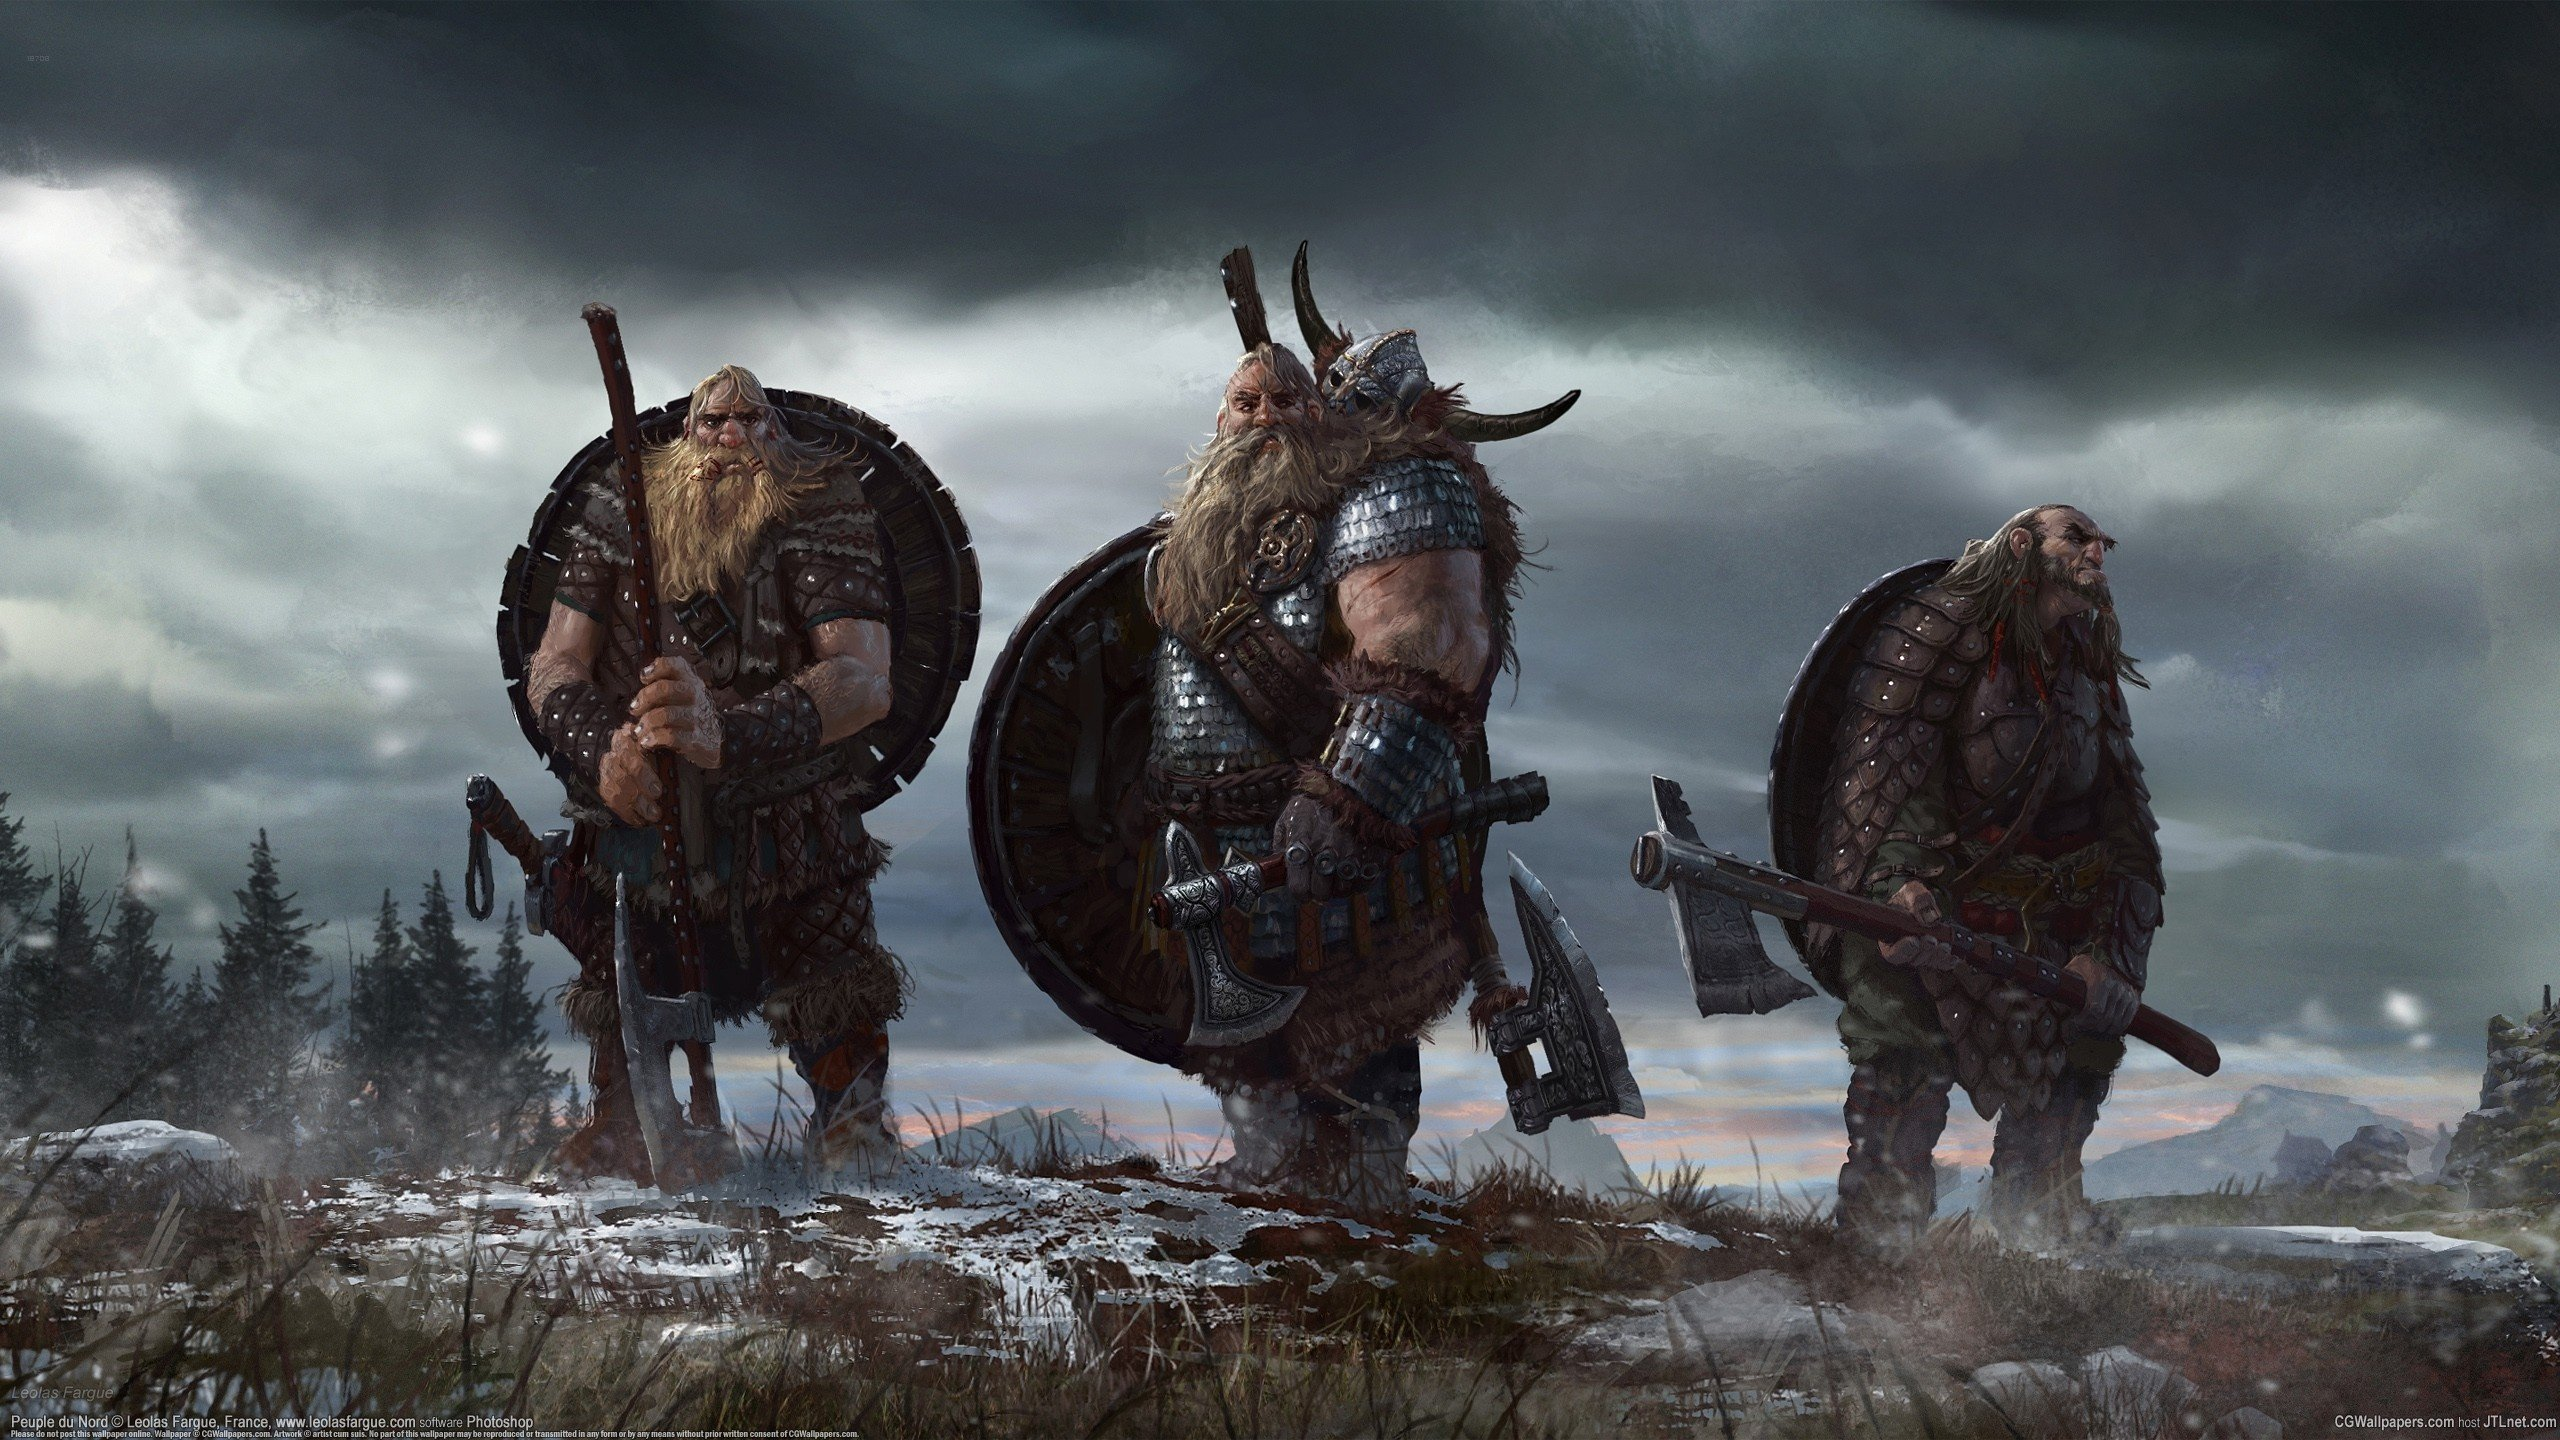
\includegraphics[width=4.5cm]{vikingwallpaper.jpg}
	\centering
	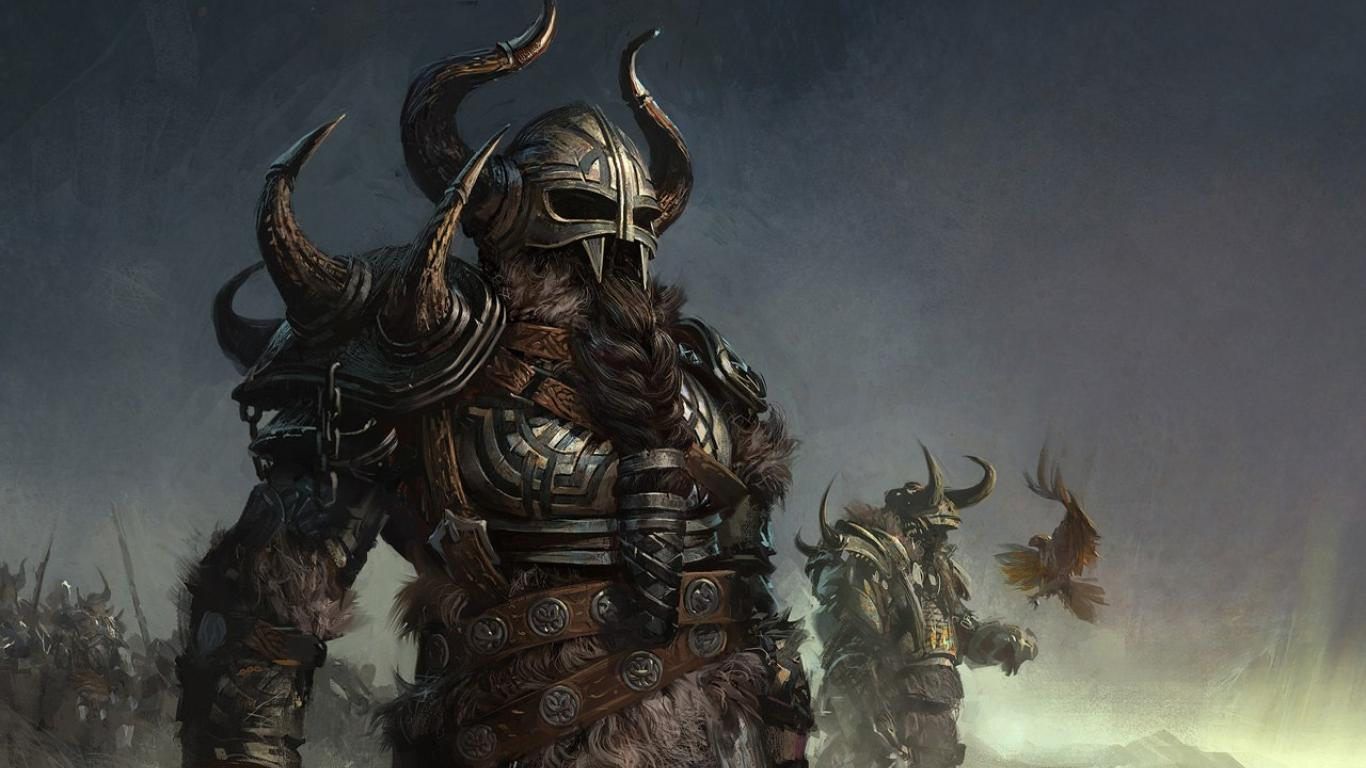
\includegraphics[width=4.5cm]{vikingwallpaper2.jpg}
	\raggedright
	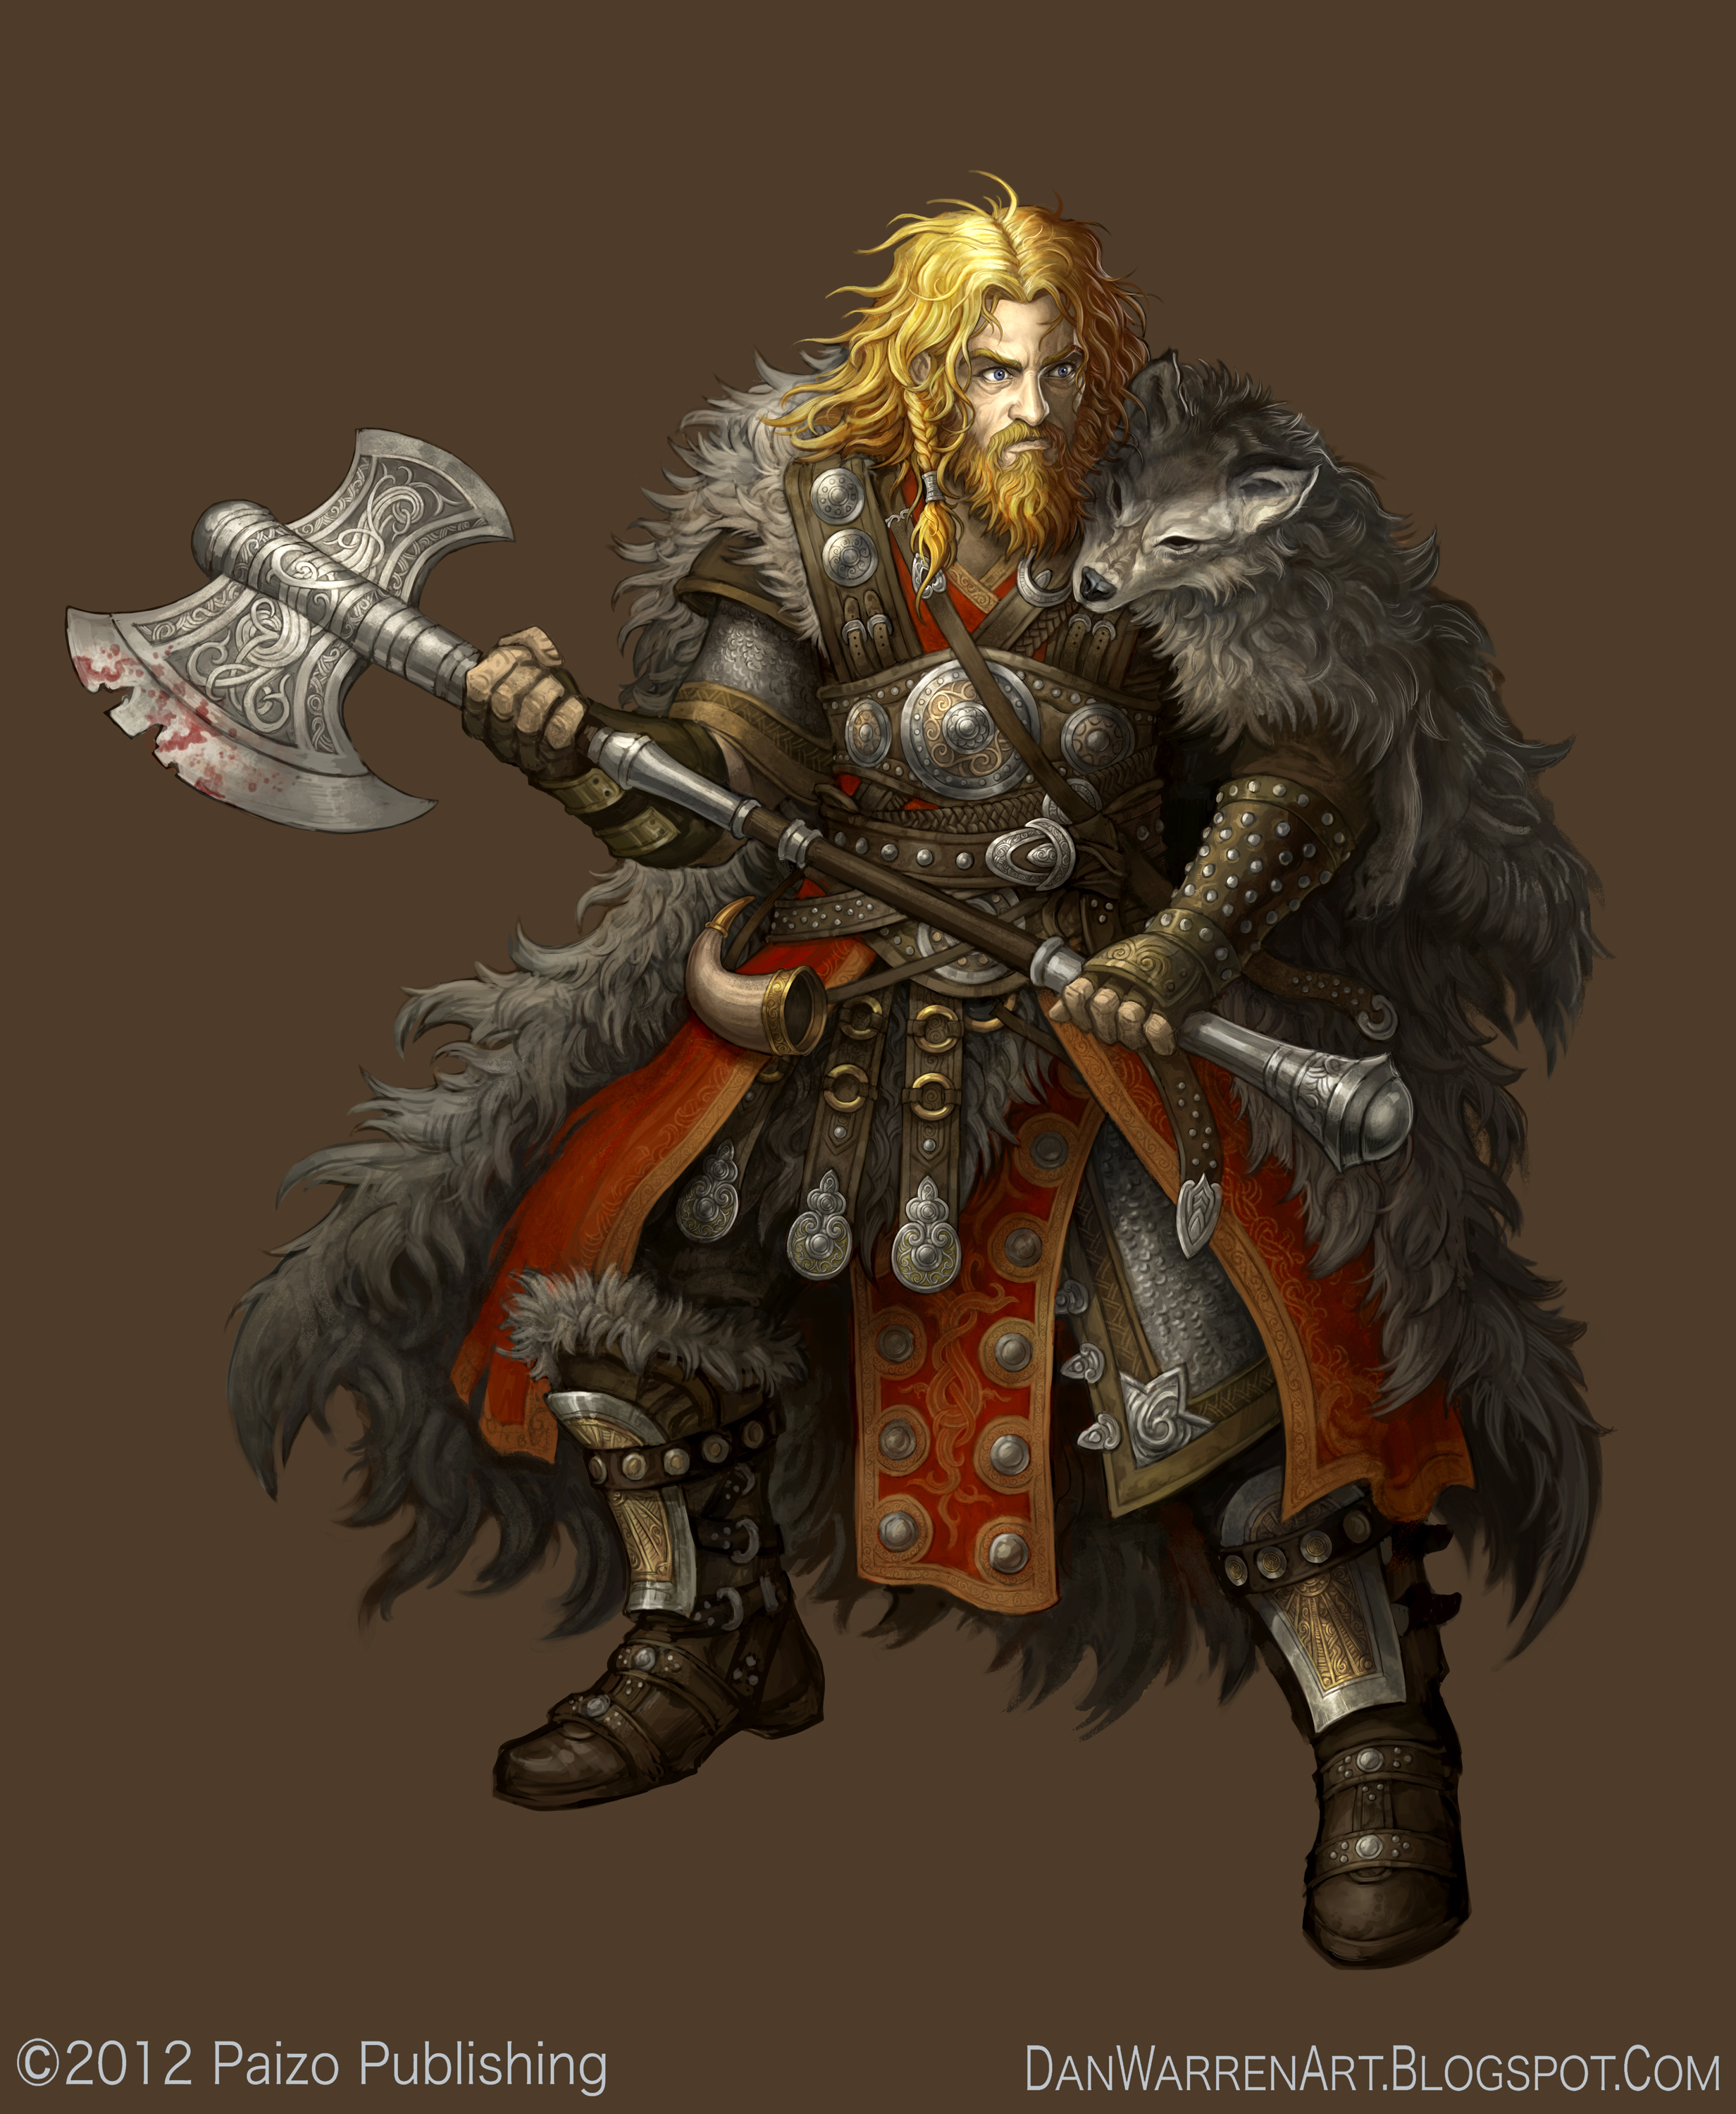
\includegraphics[width=3cm]{vikingwallpaper3.jpg}
	\caption{Vorbilder für den finalen Wikinger}
\end{figure}
\\Wikinger sind seit dem 18. Jahrhundert als noble Wilde verklärt, sie werden aber seit dem frühen 20. Jh. auch häufig als heidnische, brutale Piraten dargestellt. Attribute, die ihnen häufig zugeschrieben werden sind Wildheit, Unabhängigkeit, Kraft, Aggressivität. Darstellungen zeigen sie meistens als Krieger oder Seefahrer, oft mit Äxten und bemalten Holzschilden. Ihre Kleidung setzt sich in modernen Darstellungen aus mehreren Lagen Kleidungen oder Pelze über leichten Rüstungen wie Kettenhemden zusammen (was historisch akkurat ist), dazu die ikonischen gehörnten Helme (die historisch falsch sind). In fantastischeren Darstellungen tragen sie oft mehrere Gürtel und Medallions und gelegentlich Lamellenpanzer (Metallplättchen, die auf Leder aufgenäht werden). Wikinger tragen in modernen Darstellungen nahezu immer lange Haare und Bärte, beides häufig zu Zöpfen geflochten. 
\\Dementsprechend setzte ich den ersten Wikinger (s. Abbildung 5), der es in das finale Spiel schaffte aus mehreren dieser Elemente zusammen. Er trägt einen auffälligen gehörnten Helm, eine Axt und ein hölzernes Rundschild. Die Axt und der Helm sind bewusst vergrößert, um auch auf einem Handy-Bildschirm klar sichtbar zu sein. Die Rüstung setzt sich aus mehreren Gürtel mit Metallplättchen über einem roten Wams zusammen und wird durch Lamellenpanzer über Schulter und Waffenrock komplementiert. Die Detaildichte der Rüstung stört nicht auf dem Smartphone, da Axt, Schild und Helm den Wikinger klar erkennbar machen, sieht aber auf Tablets besser aus. Durch die Gürtel und Medallions setzt sich die Rüstung klar von "normaler" mittelalterlicher Kleidung und Rüstung ab und der Lamellenpanzer lässt ihn kriegerisch aussehen. Zusätzlich trägt er einen Pelz um die Schultern und auf den Stiefelrändern, sowie eine aus Pelz gemachte Hose, damit er etwas Wildes hat. Die Stiefel haben im Stile von Beinschienen einen metallenen Clip, um interessanter auszusehen. Dabei wurden Ränder der Figur bewusst schwarz gelassen, um die Figur vom Hintergrund abzuheben und einen Cell-Shading-Eindruck entstehen zu lassen. Später ist die Figur unser Avatar Essling auf der Karte geworden.


\newpage
\subsubsection{Der Morgenstern-Wikinger}
\begin{figure}
	\centering
	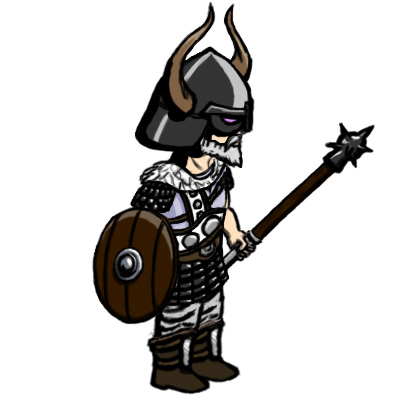
\includegraphics[height=5cm]{morningstar.jpg}
	\caption{die kühle Kolorierung mit dem Morgenstern}
\end{figure}
Da sich im Rahmen der Kolorierung des ersten Wikingers stärker mit Farblehre auseinandergesetzt wurde, entstanden danach zwei Umfärbungen, eine mit warmen und eine mit kalten Farben, unter Anderem mit dem Ziel, sie optisch stärker voneinander abzusetzen. Die Version mit den kühlen Farben bekam einen Morgenstern, eine Waffe des Spätmittelalters, um zwar aggressiv aber spezialisierter zu wirken, also bedachter. Dieser Eindruck wird verstärkt durch den weißen Bart und die generellen kühlen Farben, da kühle Farben häufig mit Rationalität in Verbindung gebracht wird.
\newpage
\begin{figure}
	\centering
	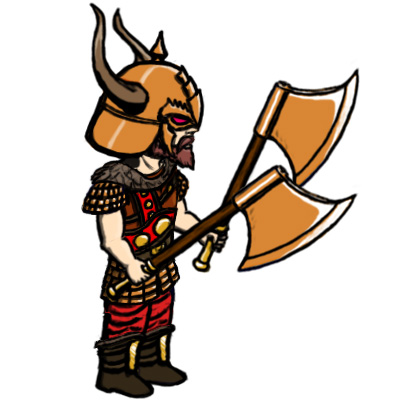
\includegraphics[height=5cm]{berserker.jpg}
	\caption{Der Berserker}
\end{figure}
\subsubsection{Der Berserker}
Die bekannteste Figur, die mit Wikingern assoziiert wird ist der Berserker, ein Krieger der sich in einen Kampfrausch versetzte. Dieser kommt in vielen Spielen vor, nicht nur in Fantasy-Wikinger-Varianten wie den Warhammer-Chaos-Berserkern, sondern auch in eher historisch angehauchten Titeln wie Age of Empires 2 und in mehreren Teilen der Civilization-Reihe. Berserker werden häufig als blutrünstig und wahnsinnig dargestellt. Dementsprechend wurde die warme Kolorierung der Berserker mit viel rot erziehlt, da rot häufig mit Aggression in Verbindung gebracht wird. Er bekam zwei Äxte, um aggressiver zu wirken und der Helm wurde nach einem Drachenkopf modelliert um die rote Assoziation mit Feuer zu verstärken und ihn stärker von den anderen beiden abzuheben. Es wurde sich dagegen entschieden, den originalen Wikinger in die finalen Kämpfe aufzunehmen, da er einen Mittelweg zwischen beiden darstellte und denkbar war, dass es zu Verwechslungen kommen könnte.

\newpage
\subsubsection{Die Priesterin des Ra}

\end{document}